\claude{
\section{Controlled experiments: recovering component structure}\label{sec:controlled}
We first test whether MG reflects the component structure that motivates the method. Analytic signals provide known dimensions; controlled learning problems test the effect of parameter updates; trained generators test whether a single neuron reveals the phase structure of a learned task. Section~\ref{sec:applied} then evaluates monitoring in applied learning problems.

\subsection{Analytic oscillators and controlled learning}
\paragraph{Known phases.}
In the analytic baseline, $r$ diagonal entries of a matrix oscillate at rationally independent frequencies. The trajectory therefore has $r$ independent phases. MG computed from a scalar observation tracks this count over $r=1$--$8$, with mean absolute error 0.27. This establishes recovery against a known geometric target before introducing learning.

\paragraph{Learning on MLP features.}
A multilayer perceptron (MLP) with tanh activations is trained on handwritten digits \citep{pedregosa2011scikit}. We freeze its features and train a linear classifier in a fixed parameter subspace. Quasiperiodic changes in the loss weights of data groups provide a controlled source of recurrent motion. We select estimator settings on separate seeds and ranks, then evaluate ranks $1,3,5,8$ on new seeds.

Every usable observable orders the held-out ranks correctly with these fixed settings. Parameter norm and fixed-probe loss stop varying when the learning rate is zero, confirming that their variation requires learning. The mean absolute error against the independently measured covariance reference is 0.90 across rank--seed--observable combinations. This reference checks the excitation of parameter directions; it is not an exact active-dimension label. The result supports accurate ordering in a controlled learning task without retuning the estimator for each rank. Appendix~\ref{app:controlled} gives errors for individual observables and distinguishes this task from earlier driven-target tests.

\paragraph{Endogenous oscillations in a regression problem.}
We next test whether MG detects fewer modes when all parameters remain trainable. We train all 32 weights of a dense linear regressor using full-batch heavy-ball updates. Repeated Hessian eigenvalues form $r$ groups; momentum one produces $r$ independent oscillatory modes with a fixed target. Selective damping reduces four modes to two without changing the data or trainable parameter count. MG of the training loss falls from 4.97 to 2.56. Multiplying the original loss by 0.01 leaves MG unchanged. The estimate therefore responds to the removal of modes in this experiment, while remaining insensitive to uniform rescaling. This is a controlled oscillatory optimizer: without damping, it oscillates around the solution rather than converging.

\subsection{Learned generators distinguish phases from harmonics}\label{sec:generator}
The next test asks whether one neuron's activity reveals the component structure learned by a recurrent network. A 1,000-unit rate network is trained by FORCE with recursive least squares \citep{sussillo2009generating} to generate one to four sinusoidal outputs. Feeding the outputs back into the network makes the learned readout affect its dynamics. At evaluation, the weights are fixed and the network runs without the target signal.

We train seven tasks on each of five seeds: one to four independent frequencies (T1--T4), two or four harmonics of one frequency (H2, H4), and two independent frequencies with their harmonics (M4). Their target phase counts are $1,2,3,4,1,1,2$, respectively. All 35 networks meet the output-fidelity criterion. A Lyapunov analysis checks the learned dynamics independently. We choose MG settings on the target signals before analyzing the networks and use neuron zero as the primary observable.

\begin{figure*}[t]
\centering
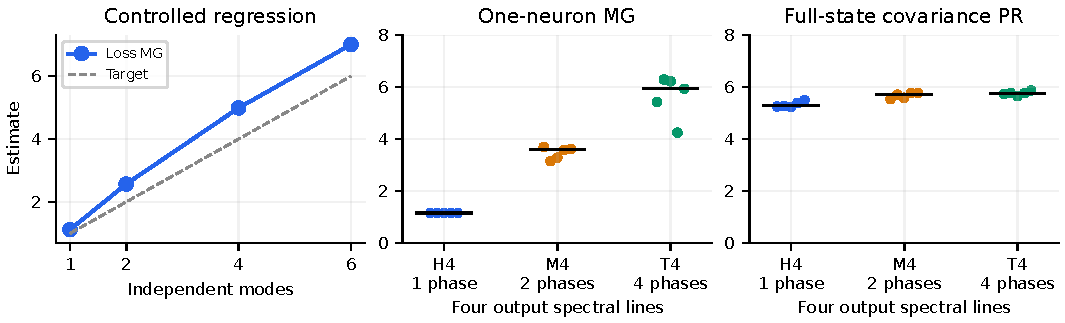
\includegraphics[width=.98\textwidth]{figures/components.pdf}
\caption{\claude{MG detects component structure from scalar records. Left: regression with a known number of modes and fixed estimator settings across ranks. Center: learned generators with four output spectral lines but one (H4), two (M4), or four (T4) independent target phases; each dot is a seed. MG separates these tasks. Right: their full-state covariance participation ratios are similar. The comparison shows sensitivity to phase structure, which differs from the spread of variance measured by participation ratio.}}
\label{fig:components}
\end{figure*}

The harmonic controls demonstrate the benefit of geometric analysis (Figure~\ref{fig:components}). H4 has four spectral lines but median MG is 1.15, close to the single-phase T1 task. For every seed, MG is lower for H2 than T2 and increases from H4 to M4 to T4. The latter three tasks have identical spectral peak counts and similar full-state covariance participation ratios: 5.27, 5.71, and 5.76. Their MG values are 1.15, 3.58, and 5.93. A single neuron's temporal record thus distinguishes phase structures that these two summaries do not separate.

Across T1--T4, median MG is 1.15, 2.84, 5.90, and 5.93. It separates one- and two-phase tasks from the higher-dimensional tasks, but does not resolve T3 from T4. The upward bias at higher phase counts limits absolute recovery at this record length. The reproducible result is discrimination of phase structure from one neuron, including the harmonic comparisons on all five seeds.

\subsection{Learning a cycle from chaotic activity}\label{sec:force}
In a separate FORCE experiment, a 256-unit network learns to produce a figure-eight trajectory from initially chaotic activity. The target has two outputs but one fundamental phase. We select five chaotic initializations using a pretraining Lyapunov criterion, without inspecting MG, and evaluate the network at saved checkpoints.

Single-neuron MG falls from 3.56--5.07 before training to 1.08--1.13 afterward in all five networks. The decline persists across three neurons and the tested window and lag settings. Independently, the full Lyapunov spectrum loses its clearly positive exponents. Four networks meet the stricter stable-cycle criterion; the fifth has weak contraction transverse to the cycle.

Both analyses identify simplification of the learned activity. MG does so from one neuron, while the spectrum uses the full state and tangent dynamics. Section~\ref{sec:cost} compares their computational costs. Here the measured trajectory is network activity at fixed weights, not the sequence of weight updates.
}
